\documentclass[t,10pt]{beamer}
\usetheme[official=true,titlebgimage=toro,conference=\mbox{N. Vianello
  @ KTH 22 June 2011}]{rfx}
\usepackage[english]{babel}
\usepackage{listings,amsmath,multimedia}
\usepackage{tangocolors}
\usepackage{rfxcolor}
\usepackage{pgf}
\usepackage{tikz}
\usepackage[bibstyle=authoryear-comp,citestyle=authoryear-comp,labelyear=true,maxnames=1]{biblatex}
\bibliography{biblio}
\renewcommand*{\bibfont}{\footnotesize}
%\renewcommand*{\citefont}{\footnotesize}
\mode<presentation>
\graphicspath{{pdf_box/}}


% for adding foot note with reference
\makeatletter
% add a macro that saves its argument
\newcommand{\footlineextra}[1]{\gdef\insertfootlineextra{#1}}
\newbox\footlineextrabox

% add a beamer template that sets the saved argument in a box.
% The * means that the beamer font and color "footline extra" are automatically added. 
\defbeamertemplate*{footline extra}{default}{
    \begin{beamercolorbox}[ht=2.25ex,dp=1ex,leftskip=\Gm@lmargin]{footline extra}
    \insertfootlineextra
    %\par\vspace{2.5pt}
    \end{beamercolorbox}
}

\addtobeamertemplate{footline}{%
    % set the box with the extra footline material but make it add no vertical space
    \setbox\footlineextrabox=\vbox{\usebeamertemplate*{footline extra}}
    \vskip -\ht\footlineextrabox
    \vskip -\dp\footlineextrabox
    \box\footlineextrabox%
}
{}

% patch \begin{frame} to reset the footline extra material
\let\beamer@original@frame=\frame
\def\frame{\gdef\insertfootlineextra{}\beamer@original@frame}
\footlineextra{}
\makeatother

\setbeamercolor{footline extra}{fg=structure.fg}% for instance

\title{Fluctuation data analysis in Fusion Relevant Plasmas\\
{\small Extracting information on relevant underlying dynamics}}
\author{N. Vianello }
\date{22 June 2011}

\begin{document}

\begin{titleframe}
\end{titleframe}

\begin{frame}
\frametitle{Motivation \& Outline}
\vspace*{\stretch{1.5}}
\only<1-5>{
Diagnostics provides information with different time and spatial resolution
\setbeamercovered{transparent=30}
\begin{enumerate}[<+-|alert@+>]
\item Measurements coming from a single point  
\item Spatially distributed arrays of measurements (resolving portion
  of the plasma or entire torus)
\item line integrated measurements (single Line Of Sight (LoS)) 
\item Arrays of LoS (examples are tomographic reconstruction)
\end{enumerate}
}

\only<5>{
\alert{We will focus on analysis technique suitable for
  single-point/multi point measurements, extracting information on
  spatial/temporal dynamics}

}
\end{frame}
\begin{frame}
\frametitle{ Continuos and Discrete Fourier transform}
\begin{itemize}[<+-|alert@+>]
\item Generally theories are developed in the frequency/wavevector
  domains ($\omega,\mathbf{k}$) rather than in time/space ($t,r$)
\item The reason for that resides principally on the fact that
  \emph{Fourier transform} of governing equation allows an easier
  treatment of typical mathematical operator
\begin{equation*}
\frac{\partial}{\partial t} \Longrightarrow i\omega; \qquad
\frac{\partial f}{\partial x_i} \Longrightarrow i k_i \hat{f}(\mathbf{k},t)
\end{equation*}
\end{itemize}
\onslide<3>{

\begin{block}{}
Some remarks on basic Fourier Transform and its discrete counterpart
the Discrete Fourier Transform are mandatory
\end{block}
}
\end{frame}

\begin{frame}{Continuous and Discrete Fourier transform 2}
The \textcolor{taorange}{Direct} and \textcolor{lightcyan}{Inverse}
fourier transform of a generic function of time $x(t)$ is defined as :
{\small \begin{equation*}
\tikz[baseline=(t1.base)]{\node[fill=taorange](t1){%
$X(f) = \int_{-\infty}^{+\infty}x(t)e^{-2\pi i f t}\mathrm{d}t$};} \qquad
\tikz[baseline=(t1.base)]{\node[fill=lightcyan](t1){%
$x(t) = \int_{-\infty}^{+\infty}X(f)e^{2\pi i f t}\mathrm{d}f$};}
\end{equation*}}
Various theorems may be applied to FT
\only<2>{
\begin{theorem}{\underline{Similarity Theorem:}}
If $x(t)$ has the Fourier transform $X(f)$ then $x(at)$ has the
Fourier Transform $|a|^{-1}F(f/a)$
\end{theorem}
\textcolor{taplum}{This will be useful in the analysis of scaling properties of the fluctuations}
}

\only<3>{
\begin{Theorem}{\underline{Addition Theorem:}}
If $x(t)$ and $g(t)$ have FT respectively $X(f)$ and $G(f)$ then
$x(t)+g(t)$ has Fourier transform $X(f)+G(f)$
\end{Theorem}
\textcolor{taplum}{The linearity of Fourier transform allows an easy
  treatment of linear equation in the Fourier domain}
}

\only<4>{
\begin{Theorem}{\underline{Shift theorem:}}
If $x(t)$ and $g(t)$ have FT respectively $X(f)$ then $x(t-a)$ has
Fourier transform $e^{-2\pi i af}X(f)$
\end{Theorem}
}

\only<5>{
\begin{theorem}{\underline{Convolution theorem:}}
If $x(t)$ and $g(t)$ have FT respectively equal to $X(f)$ and $G(f)$
the convolution of the two function $h(t) = \int_{-\infty}^{+\infty}x(t^{'})g(t-t^{'})\mathrm{d}t^{'}$
is equal to $X(f)G(f)$
\end{theorem}
The importance of the convolution equation resides on the fact that it
allows treatment of non-linearities as the term
$\mathbf{v}\cdot\nabla\mathbf{v}$ in the Navier-Stokes equations 
}

\only<6>{
\begin{theorem}{\underline{Rayleigh's Theorem}}
The integral of squared modulus of a function is equalt to the
integral of the squared modulus of its spectrum, i.e:
\begin{equation*}
\int_{-\infty}^{+\infty}|f(t)|^2\mathrm{d}t =
\int_{-\infty}^{+\infty}|F(f)|^2\mathrm{d}f
\end{equation*}
\end{theorem}
This is equivalent to an energy conservation law for the time or
frequency domain representation of the signal
}
\end{frame}

\begin{frame}{Discrete Signals}
\begin{itemize}[<+-|alert@+>]
\item In practice, signals are acquired using analog-to-digital
  converters, so discrete signals have to be analize
\item In discrete signal, a continuous functin$x(t)$ results in a set
  of $N$ discrete values of the form $x_n = x(n\Delta t)$ with $n=0,\ldots,N-1$
\item The total duration of the signal is equal to $T=N\Delta t$
  whereas the \emph{frequency sampling} is $f_s = \frac{1}{\Delta
    t}$.
\item A foundamental results of signal analysis is \emph{Sampling
    Theorem} which states that \textcolor{rfxcyan}{A function whose
    Fourier transform is zero for $f>f_c$ is fully specified by values
  spaced at equal intervals not exceeding $\frac{1}{2}f_c^{-1}$}
\item The \emph{Nyquist Frequency} $f_N = \frac{1}{2\Delta t}$, 
  equivalent to half ot the sampling frequency, thus define the
  maximum frequency which can be properly resolved, or equivalently
  given the frequency of the system we would like to investigate, we
  had to sample at least at twice the values of this frequency.
\end{itemize}
\end{frame}

\begin{frame}{Discrete Fourier Transform}
\setbeamercovered{transparent=30}
\begin{itemize}[<+->]
\item Given the discretiness of the sampling, also the corresponding
  Fourier transform will be discrete in the Fourier space.
\item The basic concept of DFT resides on the fact that the algorithm
  applied on an $N$-sampled data, will produces an information on
  $N$ frequencies, assuming that the information is conserved
\item The Fourier transform of a digitized $N$-sampled data will be of
  the form $f_n = n\Delta f$ with (if $N$ is even) $ -\frac{N}{2}\leq
  n \leq \frac{N}{2}$. The frequency resolution, in order to span all
  the allowed frequency range will be of the form $\Delta f =
  \frac{1}{T} = \frac{1}{\Delta t}$
\item The \textcolor{taorange}{Direct} and \textcolor{cyan}{Inverse}
  Discrete Fourier transform are then defined as 
{\small \begin{equation*}
\tikz[baseline=(t1.base)]{\node[fill=taorange](t1){%
$X_n = \frac{1}{N}\sum_{k=0}^{N-1}x_ke^{-2\pi kn/N}$};} \qquad
\tikz[baseline=(t1.base)]{\node[fill=cyan](t1){%
$x_k = \frac{1}{N}\sum_{n=-N/2}^{N/2}X_ne^{2\pi kn/N}$};}
\end{equation*}}

\end{itemize}

\end{frame}

\begin{frame}{Aliasing, leaking and windowing}
\only<1>{
\begin{itemize}
\item The presence of frequency higher than the Nyquist frequency may
  lead to the presence of spurious frequency
\end{itemize}
\centering{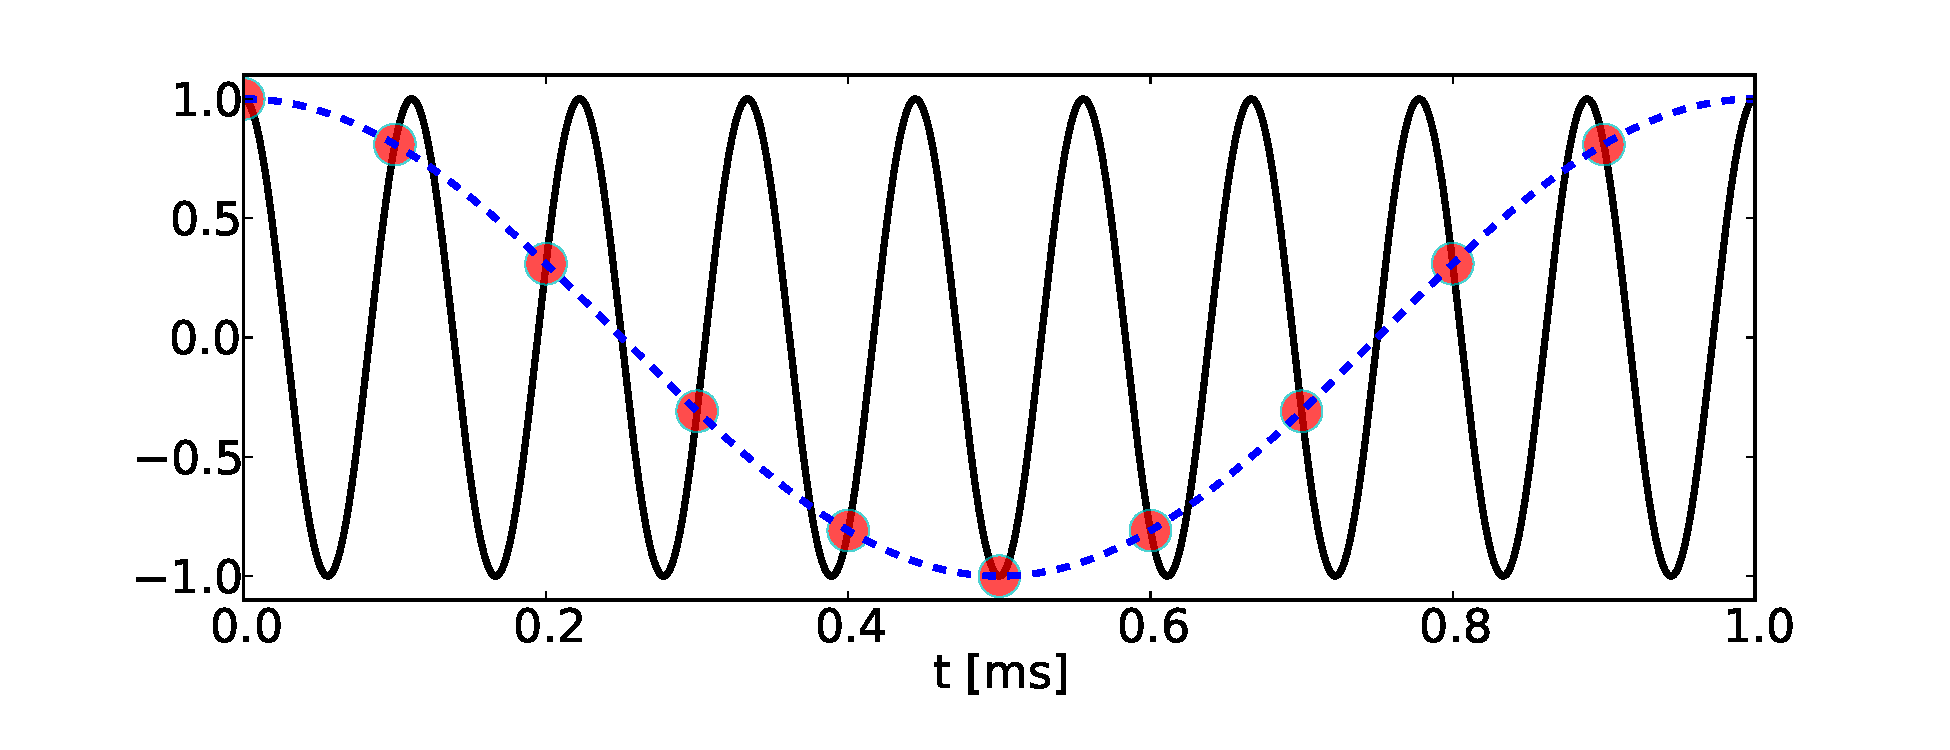
\includegraphics[width=0.6\textwidth]{aliasing}}
\begin{itemize}
\item A 9 kHz sine if sampled at 10 kHz exhibits a spurious 1 kHz oscillation
\end{itemize}
}

\only<2>{\small 
\begin{itemize}
\item The finite extension of the measurements, acquired for a given period
$T$ is equivalent to the convolution of the signal with a box
function $G(t)$ with domain $0\leq t \leq T$, i.e. $G(t)=1 $if$
0\leq t \leq T$ 0 otherwise
\item According the theorems for the Fourier transform (which can be
  applied also for discrete transform) this is equivalent in the
  Fouirer space to the moltiplication of the of the fourier transform
  but the Fourier representation of a box function is $\mathrm{sinc}(x) =
  \sin(x)/x$ function as shown, which\alert{leaking} some power from
  one frequency bin to the adjacents ones.

\centering{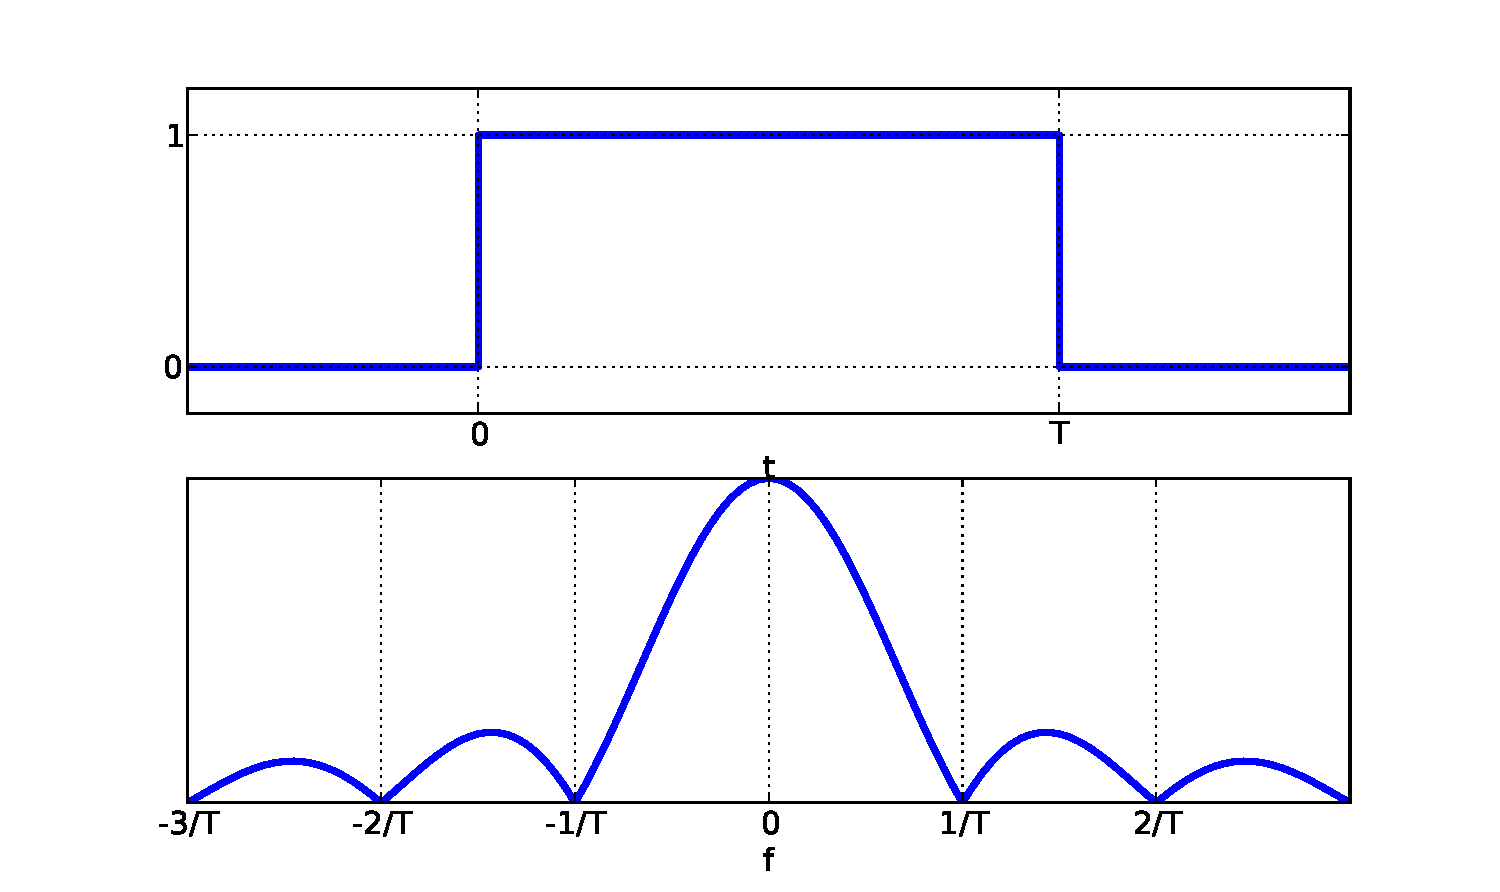
\includegraphics[width=0.5\textwidth]{box-function}}

\end{itemize}

}

\only<3>{
\begin{itemize}
\item Solution to the lakage problem is multiplying data by an
  appropriate window function which reduces the lobes as the
  \emph{Hanning window} defined as $u_h(t) = \frac{1}{2}(1-\cos(2\pi
  t/T))$ for $0\leq t\leq T$ and 0 otherwise. Its behavior in real and
  fourire space is the following 

\centering{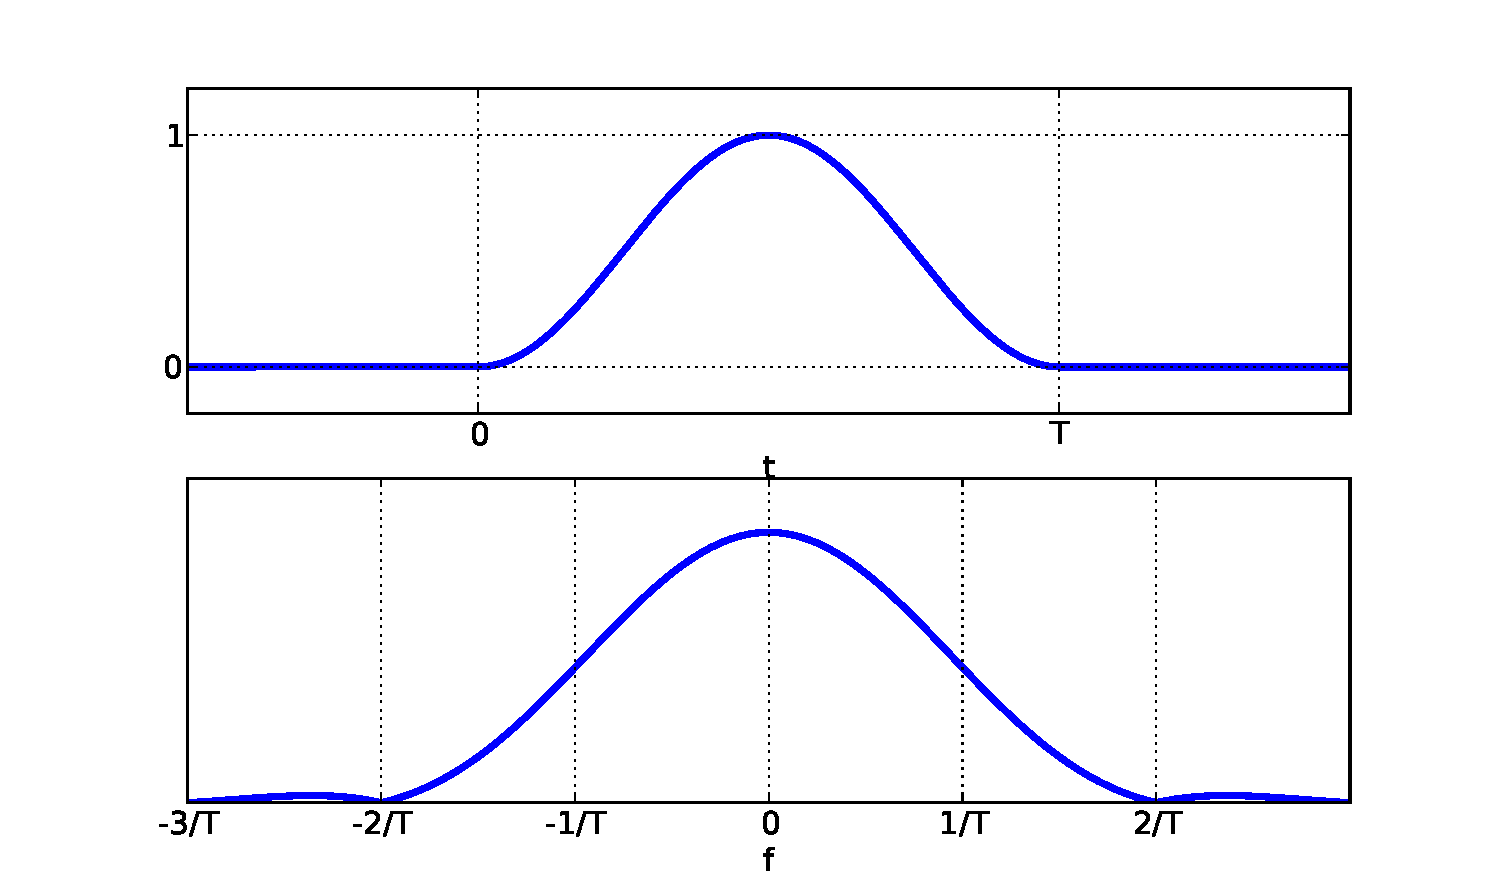
\includegraphics[width=0.5\textwidth]{Hanning}}

\end{itemize}
}
\end{frame}

\begin{frame}{Single Point: the autocorrelation function}
\begin{itemize}
\item We know from the statistics a random process $x(t)$ is
  completely described by its moments, which are the average over the
  probability distribution function 
\begin{equation*}
E|x(t)| \quad
E|x(t_1)x(t_2)| \quad
E|x(t_1)x(t_2)x(t_3)| \quad
\ldots
\end{equation*}
\item The \textcolor{taskyblue}{Auto-correlation function}, i.e. 
  the second order momentum of the distribution, or the  \textcolor{tachameleon}{autocovariance
  function }
{\small \begin{equation*}
\tikz[baseline=(t1.base)]{\node[fill=taskyblue](t1){%
$R(\tau)= E|x(t)x(t-\tau)|$};} \qquad
\tikz[baseline=(t1.base)]{\node[fill=tachameleon](t1){%
$C(\tau) = E|(x(t)-m)(x(t-\tau)-m)|$};}
\end{equation*}}
being $m$ the average of $x(t)$
\item The \textcolor{ta3orange}{Auto-correlation coefficient factor}
  is defined as $\rho(\tau)=C(\tau)/C(0)$
\item For digitized signals with $N$ samples the estimator of
  $C(\tau)$ is defined as 
{\small \begin{equation*}
C_j =
\frac{1}{N}\sum_{i=j}^{N-1}(x_i-\overline{x})(x_{i-j}-\overline{x})
\qquad \overline{x}=\frac{1}{N}\sum_{i=0}^{N-1}x_i
\end{equation*}}
\end{itemize}
\end{frame}

\begin{frame}{Auto-correlation: practical use}
\begin{itemize}
\item Define the \textcolor{ta3plum}{\emph{Auto-correlation time}} of
  a turbulent field such as the potential
\item \textbf{Inserisci figura con autocorrelazione di un potenziale }
\end{itemize}
\end{frame}

\begin{frame}{Single point: the power spectrum}
\begin{itemize}[<+->]
\item The \textcolor{ta3skyblue}{Power spectrum $S(f)$} is defined as the
  Fourier transform of the Autocorrelation-function.
\item It can be demonstrated that
  $E[|x(t)|^2]=\int_{-\infty}^{+\infty}S(f)dt$, i.e. the Power
  spectrum describe the frequency distribution of the \emph{power of
    the signal.}
\item In the real case, with limited temporal acquisition of a signal $x_T(t)$
  the ensemble average of its \textcolor{ta3skyblue}{periodogram}
  tends to the power spectrum
  $\frac{|FT(x_T(t))|^2}{T}\xrightarrow[T\rightarrow \infty]{} S(f)$
\item From a practial point of view, we divide
  signals into $M$ slices, assumed as indipendent realization of the
  same stochastic process and we compute
\begin{equation*}
\hat{S}(f) = \frac{1}{M}\sum_{k=1}^{M} S^{(k)}(f) ; \qquad S^{(k)}(f)=\frac{1}{T}|X_T^{(k)}(f)|
\end{equation*}
\item With digitized signal, the power spectral estimator $\hat{S}_n$
  is related to the real power spectrum $S(f_n)$ as 
\begin{equation*}
\hat{S}_n = \frac{1}{M}\sum_{k=1}^{M}|X_n^{(k)}|^2; \qquad \hat{S}_n
\simeq S(f_n)\Delta f
\end{equation*}
\end{itemize}
\end{frame}

\begin{frame}{Power spectrum: practical use}
\begin{columns}[b]
\begin{column}{.5\textwidth}
\begin{itemize}
\item \textcolor{ta3scarletred}{Mode identification at a given
    frequency {\footnotesize \parencite{Conway:2005gq}}}
\end{itemize}
\end{column}
\begin{column}{0.5\textwidth}
\centering{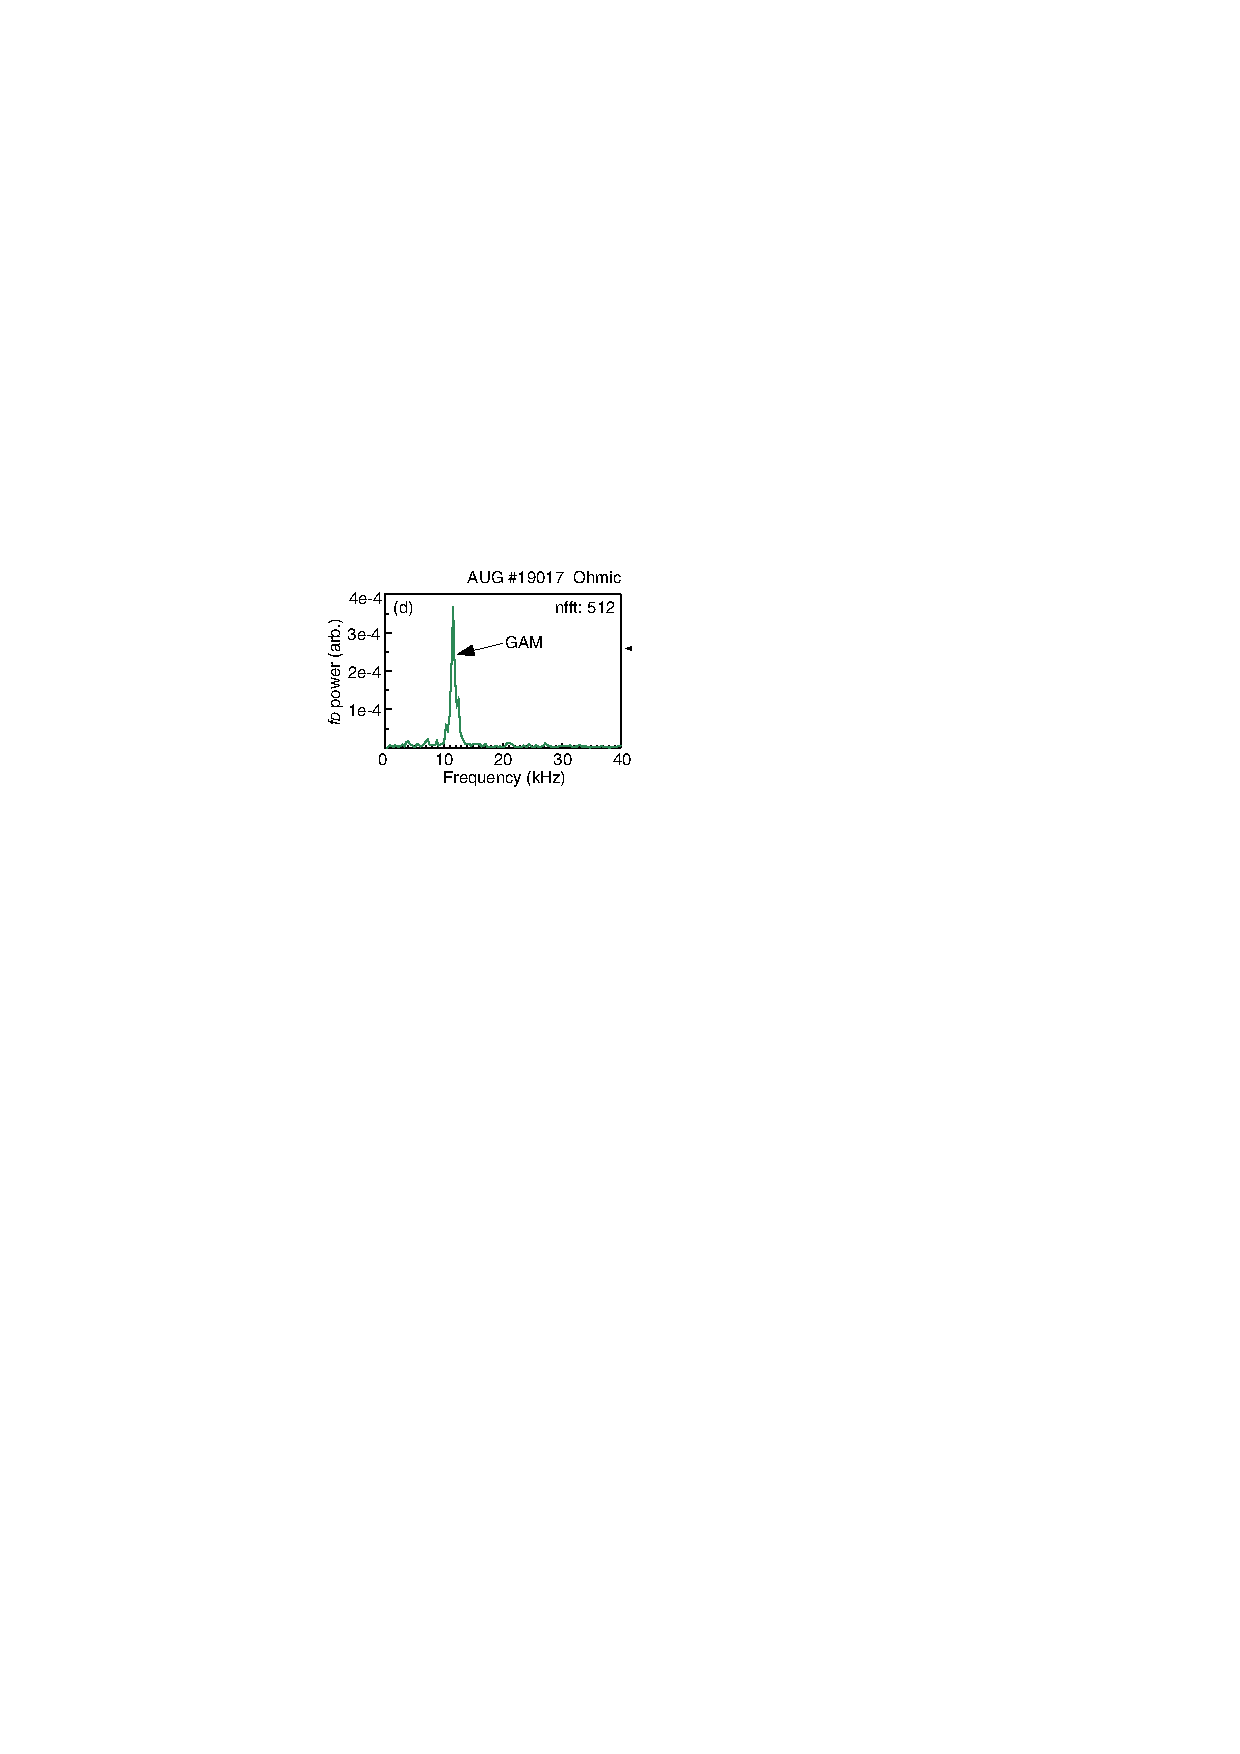
\includegraphics[width=0.9\textwidth]{gam-conway}}
%{\footnotesize G. Conway PPCF }
\end{column}
\end{columns}

\vspace{0.5cm}

\begin{columns}[b]
\begin{column}{0.5\textwidth}
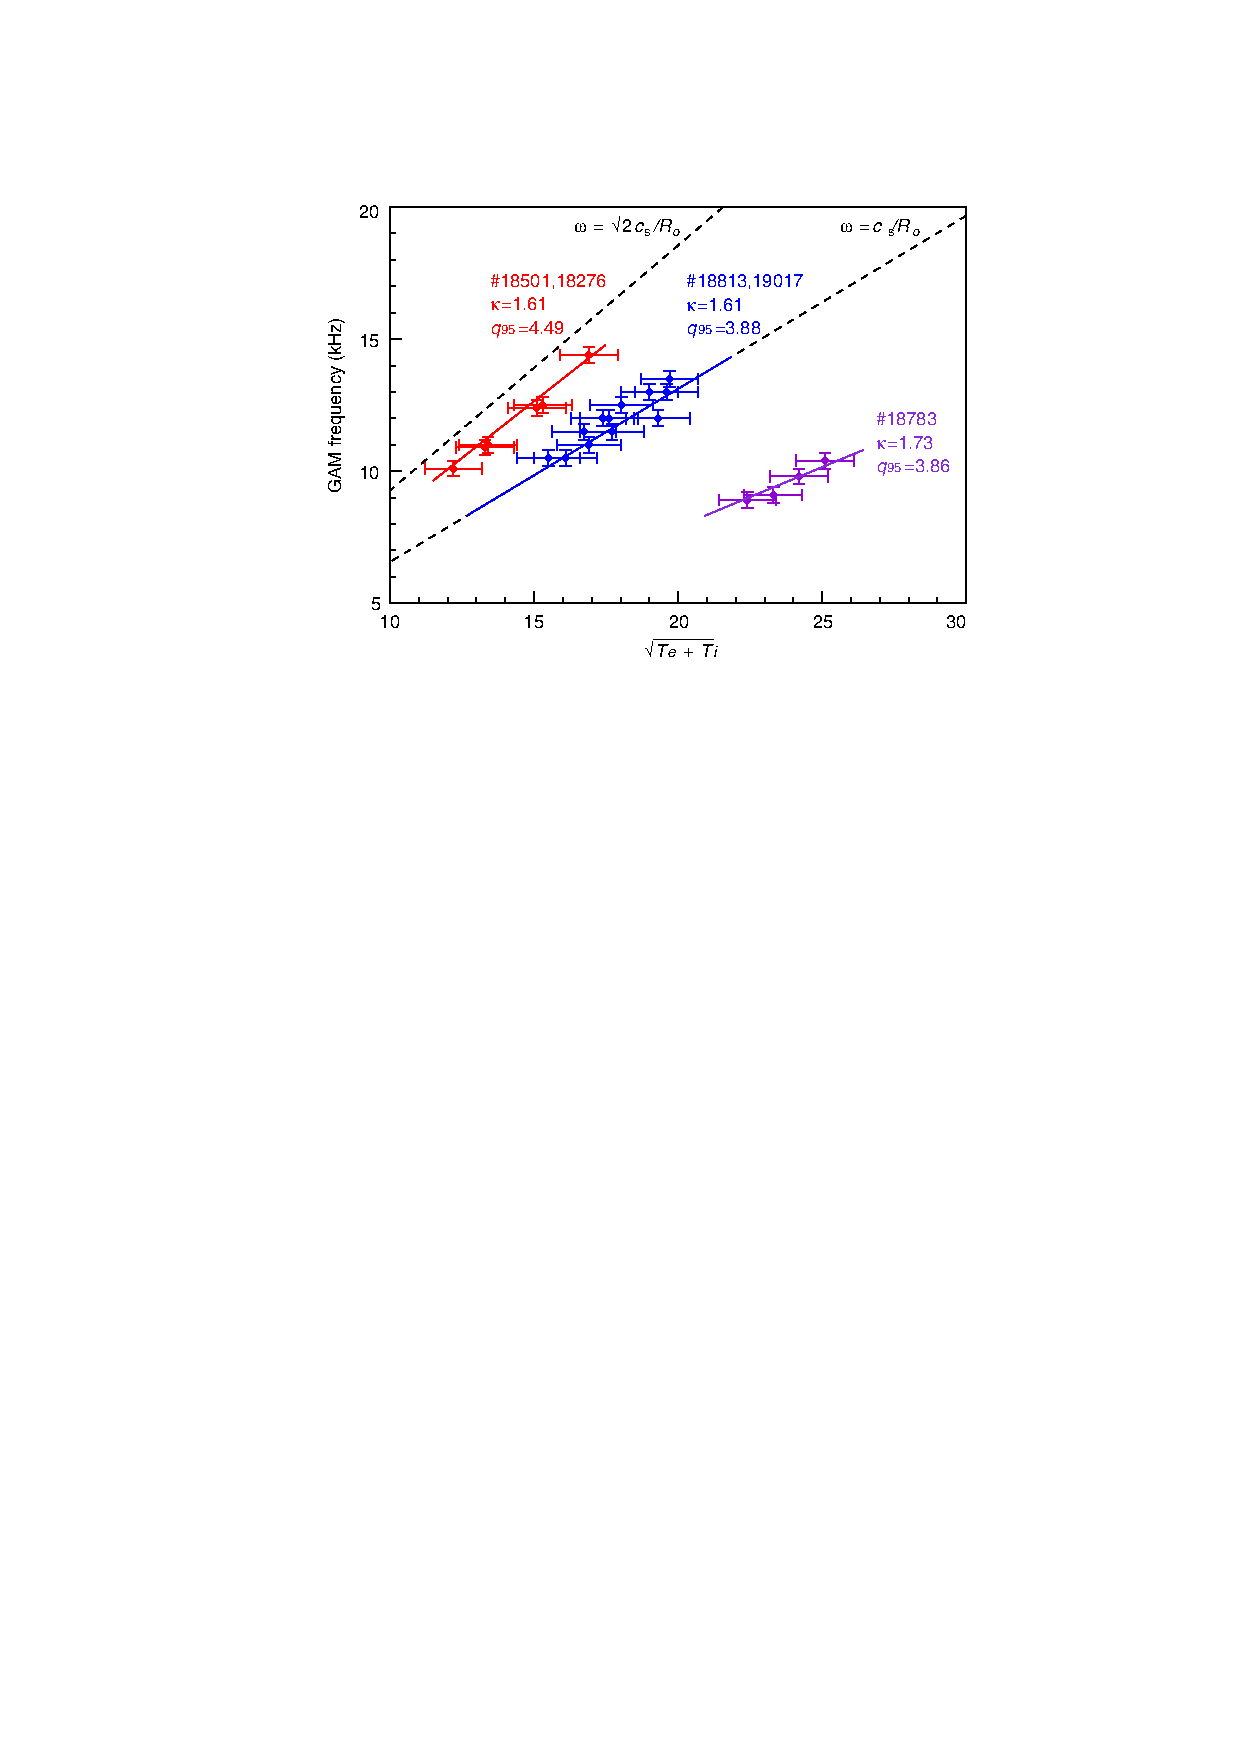
\includegraphics[width=0.8\textwidth]{gam-scaling}
\end{column}
\begin{column}{0.5\textwidth}
{\small \begin{itemize}
\item But information must be completed. In the example, precise
  identification require scaling of identified mode as a function of
  ion sound gyroradius
\end{itemize}}
\end{column}
\end{columns}
\end{frame}

\begin{frame}{Power spectrum: The spectrogram}
\begin{itemize}
{\small \item The same information can be also analyzed in time applying the
  \textcolor{tascarletred}{\texttt{spectrogram}} technique which shows
  how the spectral density of the signal varying in time/frequency
  space {\footnotesize \parencite{spagnolo}}
}\vspace{0.5cm}

\centering{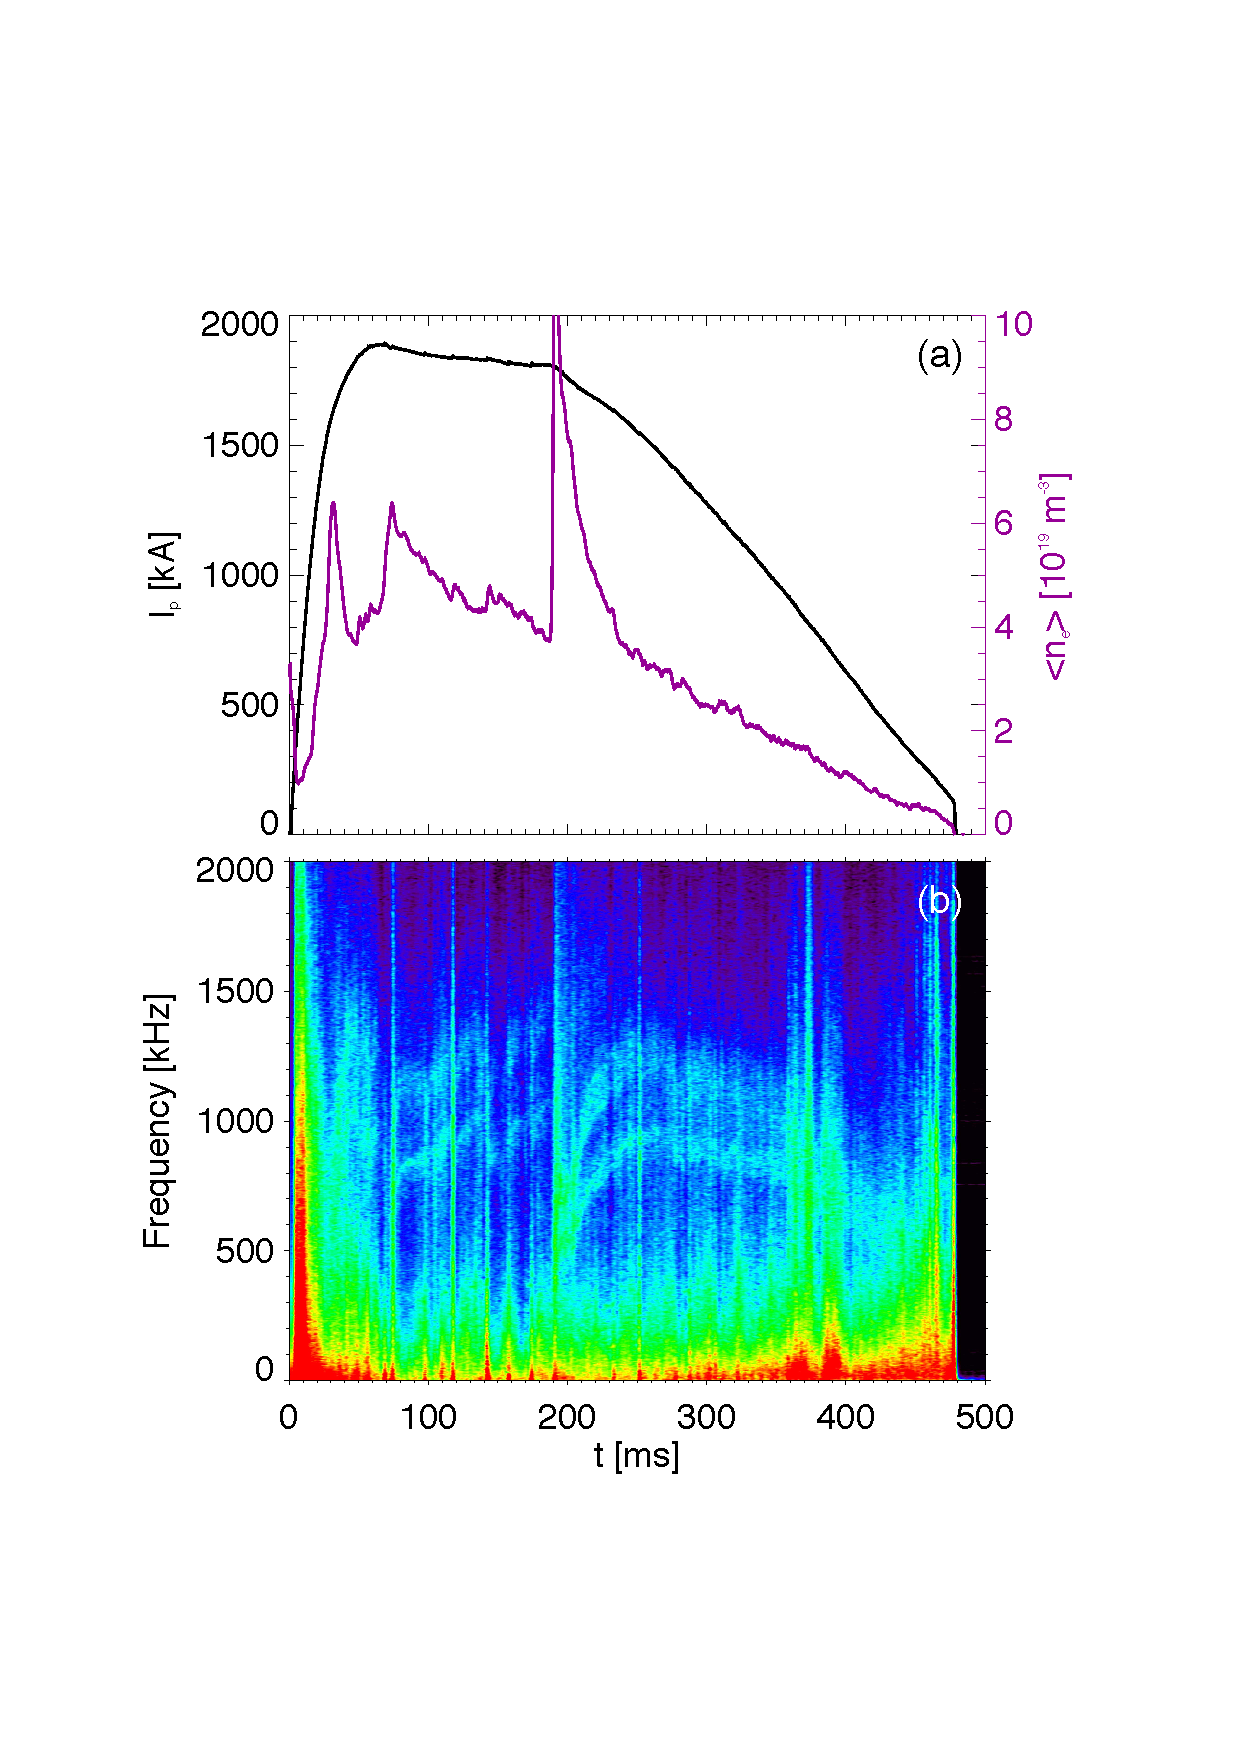
\includegraphics[height=4.5cm]{alfven} }

\item Again the information must be completed, as in the case proposed
  where the Alfv\'enic nature of the observed peaks is revealed by the
  comparison with the plasma density
\end{itemize}
\end{frame}


\begin{frame}{Two-points techniques}

\begin{itemize}[<+->]
\item Spatially distributed measurements allow access to spatial
  structure of the fluctuations
\item The minimum set includes two measurements $x(t)$ and $y(t)$. We can define the
  \textcolor{tascarletred}{Cross-correlation function},
  \textcolor{taorange}{The cross-covariance function} and the
  \textcolor{taskyblue}{cross-correlation coefficient function}
{\footnotesize \begin{gather*}
\tikz[baseline=(t1.base)]{\node[fill=tascarletred](t1){%
$R_{xt}(\tau)=E[y(t)x(t-\tau)]$};}  \\
\tikz[baseline=(t1.base)]{\node[fill=taorange](t1){%
$C_{xy}(\tau)=E[(y(t)-\overline{y})(x(t-\tau)-\overline{x})]$};} \\
\tikz[baseline=(t1.base)]{\node[fill=taskyblue](t1){%
$\rho_{yx}(\tau) = \frac{C_{yx}(\tau)}{\sqrt{C_{xx}(0)C_{yy}(0)}}$};}
\end{gather*}}
\item In the discrete counterpart of the cross-covariance is
  defined as
{\footnotesize\begin{equation*}
C_{yx,j}=\frac{1}{N}\sum_{i=j}^{N-1}(y_i-\overline{y})(x_{i-j}-\overline{x})
\end{equation*}
}
\end{itemize}
\end{frame}

\begin{frame}{Two-points technique}
\begin{itemize}[<+->]
\item In analogy to the power spectrum we define the
  \textcolor{tascarletred}{Cross-power spectrum $S_{XY}(f)$} as the
  Fourier transform of the cross-correlation function
\item As in the case of power spectrum, if $x(t)$ and $y(t)$ are real
  function, the cross-power spectrum is totally defined by the
  positive frequency only
\item Differently from the power spectrum, the cross-spectrum is
  complex-valued $S_{YX}(f)=|S_{YX}(f)|e^{i\Theta_{YX}(f)}$ with
  $\Theta_{YX}(f)$ equal to the \textcolor{tascarletred}{\texttt{Phase
    spectrum}}
\item We can also defined the
  \textcolor{tascarletred}{\texttt{coherence}} as $\gamma_{YX}(f)=\frac{|S_{YX}(f)|}{\sqrt{S_Y(f)S_X(f)}}$
\item In the case of discrete signals with finite temporal length the following definitions hold
  (in analogy to single point case)
\begin{equation*}
\hat{S}_{Y,X,n}= \frac{1}{M}\sum_{k=1}^MY_n^{(k)}X_n^{*(k)} \qquad
\hat{S}_{Y,X,n}\simeq S_{YX}(f_n)\Delta f
\end{equation*}
\end{itemize}
\end{frame}

\begin{frame}{Phase spectrum}
\begin{itemize}[<+->]
\item The method can be applied also in the case of two quantities
  measured on the same location
\item In the case of Langmuir probes for example, electron density
  $n_e$ and plasma potential $\phi_p$ are know in the same nominal
  position

\centering{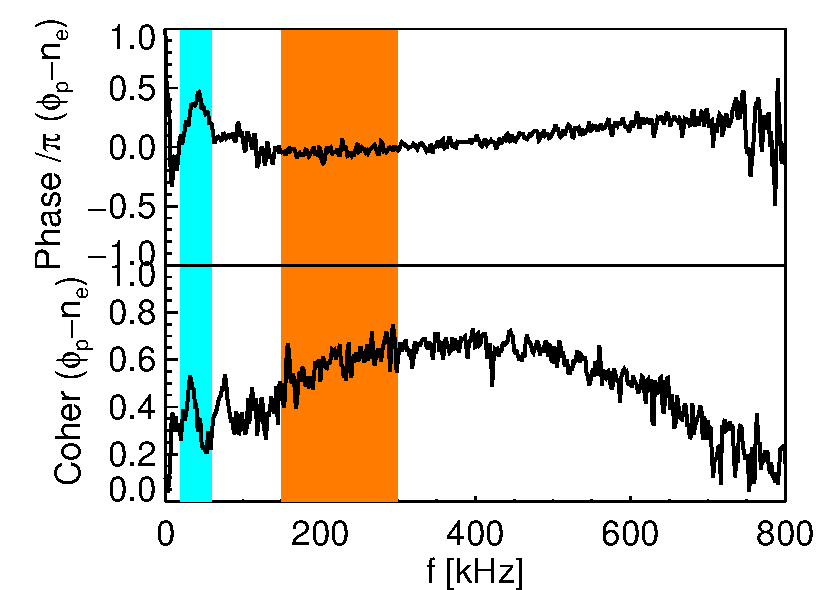
\includegraphics[height=4cm]{PhaseCoherenceEn-Vp20367}}

\item This allow the possibility to distinguish the frequency where
  turbulence is \textcolor{rfxcyan}{Interchange-dominated} from that
  where turbulence is \textcolor{orange}{Drift-dominated}
\item Other possibility is the determination of the polarization of
  magnetic fluctuations frequency resolved 
\end{itemize}
\end{frame}

\begin{frame}{Wave-vector estimate}
\begin{itemize}[<+-|alert@+>]
\item In the case of a reasonably deterministic dispersion relation between $k$ and $f$, the phase may be
  used for the determination of $k$
\item Indeed if $k = k(f)$ then at a generic position $\overline{r}$
  the function $g(t,\overline{r}) =
  \int_{-\infty}^{+\infty}G(f)e^{-ik(f)\cdot \overline{r}}e^{i2\pi f}df$
\item If measures exhists at two position $g(t,\overline{r}_1)$ and
  $g(t,\overline{r}_2)$ separated by $d$ at a given frequency the two signals will be
  phase shifted of $\Theta_{12}(f)=k(f)d$ where $\Theta_{12}(f)$ is
  computed trough the cross-power spectrum
\item If measurements are displaced in the aximuthal direction,
  i.e. $d=r_p\Delta\Theta$ then the azimuthal mode number is computed
  as $m=\Theta_{12}/\Delta\Theta$
\item \textcolor{tachameleon}{The probe distance $d$ must be less than
  aa wave length, less than a correlation lenght, but far enough the
  detect a measurable phase difference}
\end{itemize}
\end{frame}

\begin{frame}{Fluctuation-induced particle transport}
\begin{itemize}
\item Fluctuations induced particle flux is defined as $\Gamma = E[\tilde{n}(t)\tilde{v}(t)]=E[\tilde{n}(t)\tilde{E}(t)]/B$
\item According to previous definitions and properties 
\begin{equation*}
\Gamma
=\frac{1}{B}R_{nE}(\tau=0)=\frac{1}{B}\int_{-\infty}^{+\infty}S_{nE}(f)e^{i2\pi
f\tau}df = \frac{2}{B}\int_0^{+\infty}\Re[S_{nE}(f)]df
\end{equation*}
\item In quasi-static approximation $\tilde{E}=-\nabla\tilde{\phi}$,
  and considering the finitness of the measurements we
  end up with the formula
\begin{eqnarray*}
\Gamma(f) = \frac{2}{BT}\Im\{ E[k(f)N(f)\Phi^{*}(f)]\} \\
\Gamma(f)=\frac{2k(f)}{B}\Im\{S_{n\phi}(f)\} \; \text{if $k(f)$ is deterministic}
\end{eqnarray*}
\end{itemize}
\end{frame}

\begin{frame}{Fluctuation-induced particle transport 2}
\begin{itemize}
{\footnotesize
\item In practice, considering digitzed signals we have 
\begin{gather*}
\Gamma(f)=\frac{1}{M}\sum_{k=1}^{M}\Gamma^{k}(f) \\
\Gamma^{(k)}(f)=\frac{2}{B}\Im\{k^{(k)}(f)N^{(k)}(f)\Phi^{*(k)}(f)\}
 0<f<N/2-1 \\
\Gamma^{(k)}(f)=\frac{1}{B}\Im\{k^{(k)}(f)N^{(k)}(f)\Phi^{*(k)}(f)\}
 f=0,f=N/2
\end{gather*}
}
\only<2>{
\centering{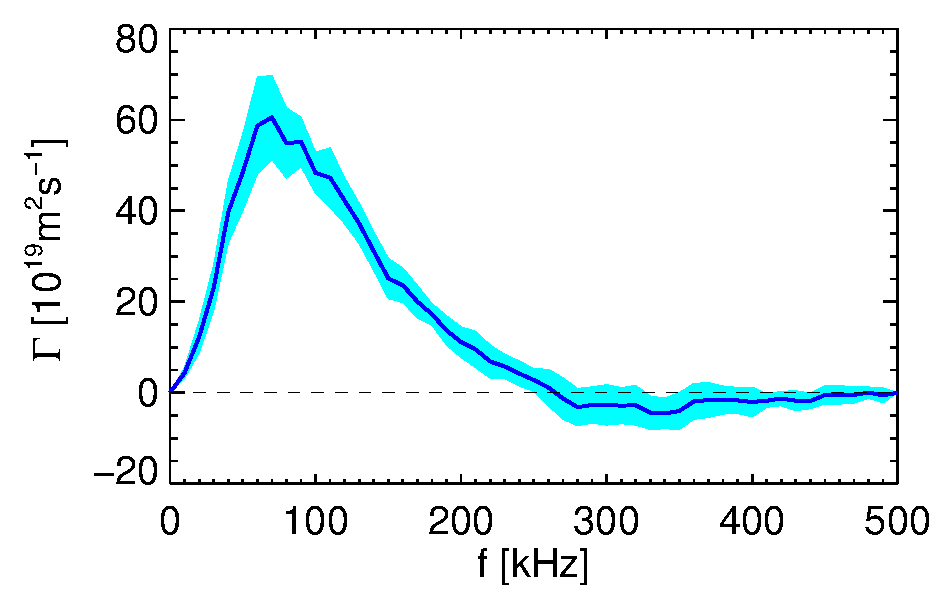
\includegraphics[height=3.5cm]{flux_vs_f}}
}

\only<3>{
\centering{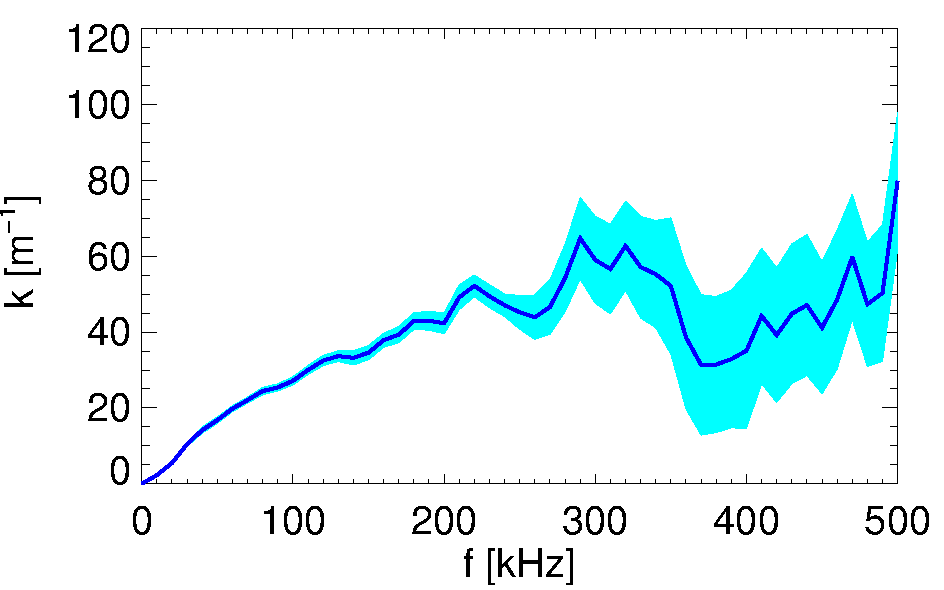
\includegraphics[height=3.5cm]{k_vs_f}}
}

\only<4>{
\centering{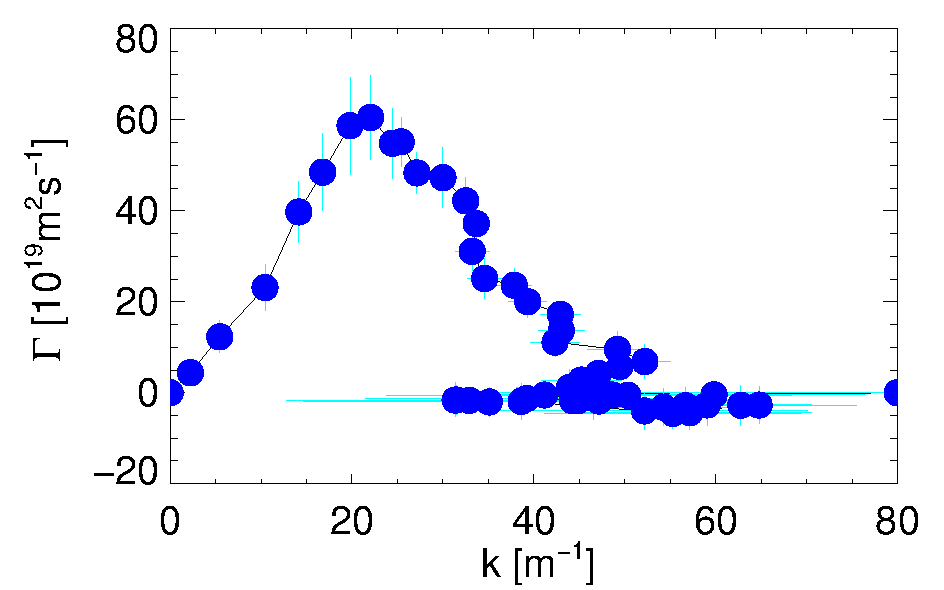
\includegraphics[height=3.5cm]{flux_vs_k}}
}

\end{itemize}
\end{frame}
\end{document}
